\documentclass[10pt, a4paper]{article}

% márgen + layout
\usepackage[a4paper, margin=3mm, top=3mm, bottom=3mm]{geometry}
\usepackage{multicol}
\setlength{\columnsep}{2mm}
\setlength{\columnseprule}{0.3pt}

% matemática
\usepackage{amsmath, amssymb, bm}

% tipografía
\usepackage{microtype}
\usepackage{parskip}
\setlength{\parskip}{0pt}
\setlength{\parindent}{0pt}

% títulos compactos
\usepackage{titlesec}
\titlespacing{\section}{0pt}{2pt}{1pt}
\titlespacing{\subsection}{0pt}{1pt}{0pt}
\titleformat{\section}{\small\bfseries\centering}{}{0em}{}[\hrule]
\titleformat{\subsection}{\footnotesize\bfseries}{}{0em}{}

% espaciado ecuaciones
\setlength{\abovedisplayskip}{1pt}
\setlength{\belowdisplayskip}{1pt}
\setlength{\abovedisplayshortskip}{0pt}
\setlength{\belowdisplayshortskip}{0pt}

% enumeración
\usepackage{enumitem}
\setlist{noitemsep, topsep=0pt, leftmargin=*}

% atajos de latex
\usepackage{physics}

% pseudocódigo
\usepackage{algorithmicx}
\usepackage{algpseudocode}
\algtext*{EndFor}
\algtext*{EndIf}
\algtext*{EndWhile}
\algtext*{EndProcedure}
\algtext*{EndFunction}

% gráficos
\usepackage{tikz}
\usetikzlibrary{angles}

% cuadros
\usepackage[most]{tcolorbox}
\tcbset{
    formulabox/.style={
        enhanced,
        colback=white,
        colframe=black!60,
        fonttitle=\bfseries\footnotesize\color{white},
        title=#1,
        boxrule=0.4pt,
        arc=1mm,
        left=1mm, right=1mm, top=1.8mm, bottom=0.5mm,
        before skip=1mm,
        after skip=1mm,
        attach boxed title to top left={yshift=-2.2mm, xshift=2mm},
        boxed title style={
            colback=tcbcolframe,
            colframe=tcbcolframe,
            boxrule=0pt,
            arc=0.6mm,
            left=0.5mm, right=0.5mm, top=0.2mm, bottom=0.2mm,
        },
        before upper={
            \raggedright\scriptsize
            \setlength{\abovedisplayskip}{1pt}
            \setlength{\belowdisplayskip}{1pt}
            \setlength{\abovedisplayshortskip}{0pt}
            \setlength{\belowdisplayshortskip}{0pt}
            },
        segmentation style={solid, line width=0.4pt},
    }
}

% colores
\usepackage[dvipsnames]{xcolor}

\definecolor{softBlue}{HTML}{7A9EB5}
\definecolor{softGreen}{HTML}{7AA882}
\definecolor{softRed}{HTML}{B57A7A}
\definecolor{softPurple}{HTML}{9A85A8}
\definecolor{softOrange}{HTML}{B8956A}
\definecolor{softTeal}{HTML}{6A9FA0}
\definecolor{softBrown}{HTML}{8C7B6B}
\definecolor{softSlate}{HTML}{7A8FA6}

% comandos personalizados
\newcommand{\w}{\mathbf{w}}
\newcommand{\x}{\mathbf{x}}
\newcommand{\X}{\mathbf{X}}
\newcommand{\y}{\mathbf{y}}
\newcommand{\z}{\mathbf{z}}
\newcommand{\del}{\boldsymbol{\delta}}
\newcommand{\bias}{\mathbf{b}}
\newcommand{\preact}{\mathbf{a}}
\newcommand{\W}{\mathbf{W}}
\newcommand{\Loss}{\mathcal{L}}
\newcommand{\muu}{\boldsymbol{\mu}}
\newcommand{\Sig}{\boldsymbol{\Sigma}}
\newcommand{\ELBO}{\text{\L}}
\newcommand{\E}{\mathbb{E}}
\begin{document}
\noindent

%%%%%%%%%%%%%%%%%%%%%%%%%%%%%%%%%%%%%%% COL 1 %%%%%%%%%%%%%%%%%%%%%%%%%%%%%%%%%%%%%%%
\begin{minipage}[t]{0.3299\textwidth}
\vspace{0pt}

% K-MEANS
\begin{tcolorbox}[formulabox=K-Means, colframe=softRed]
    \textbf{Objetivo}: $\min_{\{r_{nk}\},\{\muu_k\}} J = \sum_n\sum_k r_{nk}\|\x_n - \muu_k\|^2$ \\
    $r_{nk} \in \{0,1\}$, $\sum_k r_{nk} = 1$ (asignación \textit{hard})
    \vspace{-2mm}
    \tcbline
    \vspace{-2mm}
    \textbf{Inicialización} $\muu_k$ (random o K-Means++) \\
    $\approx$\textbf{E-Step}: $z_n^* \leftarrow \arg\min_k \|\x_n - \muu_k\|^2$ \\
    $\approx$\textbf{M-Step}: $\muu_k \leftarrow \frac{1}{N_k}\sum_{n:\,z_n^*=k}\x_n$ \\
    \textbf{K-Means++}: $p(\muu_{t+1} =\x_n) = \frac{d_{t}(\x_n)}{\sum_{n'} d_t(\x_{n'})}$\\
    $d_t(\x)=\min^{t}_{k=1} \| \x - \muu_k\|^2_2$ \\
    \textbf{Límite de GMM}: $\Sig_k = \varepsilon\mathbf{I}$, $\varepsilon\to 0$ $\Rightarrow$ asignación hard (gaussianas infinitamente concentradas).
\end{tcolorbox}

% GMM
\begin{tcolorbox}[formulabox=Gaussian Mixture Model (GMM), colframe=softRed]
    $p(\x|\w) = \sum_{k=1}^K \pi_k\,\mathcal{N}(\x|\muu_k,\Sig_k)$;\quad $\sum_k\pi_k=1$ \\
    Latente: $z \sim \text{Cat}(\boldsymbol{\pi})$; $\x|z=k \sim \mathcal{N}(\muu_k,\Sig_k)$\\
    $\ln p(\X|\w) = \sum_n \ln \sum_k \pi_k\,\mathcal{N}(\x_n|\muu_k,\Sig_k)$
    \vspace{-2mm}
    \tcbline
    \vspace{-2mm}
    \textbf{E-step} (responsabilidades, soft clust.):
    $r_{nk} = p(\z = k \mid x_n, \boldsymbol{\theta})= \dfrac{\pi_k\,\mathcal{N}(\x_n|\muu_k,\Sig_k)}{\sum_{k'}\pi_{k'}\,\mathcal{N}(\x_n|\muu_{k'},\Sig_{k'})}$\\[2pt]
    \textbf{M-step}:\\
    $N_k = \textstyle\sum_n r_{nk}$;\quad
    $\hat{\pi}_k = \tfrac{N_k}{N}$;\quad
    $\hat{\muu}_k = \tfrac{1}{N_k}\sum_n r_{nk}\x_n$\\
    $\hat{\Sig}_k = \tfrac{1}{N_k}\sum_n r_{nk}(\x_n{-}\hat{\muu}_k)(\x_n{-}\hat{\muu}_k)^\top$\\[2pt]
    \textbf{Asignación} (hard clust.): $\z_n = {\arg \max}_k r_{nk}$ \\
    \textbf{Frontera GMM}:$r_{nk} = r_{nk'}$, lineal si $\Sig_k=\Sig \forall k$.
\end{tcolorbox}

% ELBO + EM
\begin{tcolorbox}[formulabox=EM \& ELBO, colframe=softTeal]
    \textbf{Goal}: $\max_\w \ln p(\x|\w) = \max_\w \ln\sum_\z p(\x,\z|\w)$ \\[2pt]
    Asumiendo $q(\z)$:
    \begin{align*}
        \ln p(\x|\w) &= \underbrace{\E_{q(\z)}\!\left[\ln \tfrac{p(\x,\z|\w)}{q(\z)}\right]}_{\ELBO(\w,\,q)} + \underbrace{D_\mathbb{KL}(q(\z)\|p(\z|\x,\w))}_{\geq 0}\\
        \ln p(\x|\w) &\geq \ELBO(\w, q)
    \end{align*}
    \textbf{E-step}: Maximizar $\ELBO$ respecto a $q$\\
    $q^* = p(\z|\x,\w^{t-1})$ $\Rightarrow$ KL$=0$, $\ELBO=\ln p$\\
    \textbf{M-step}: Maximizar $\ELBO$ respecto a $\w$\\
    $\w^t = \arg\max_\w\,\mathbb{E}_{q(\z)}[\ln p(\x,\z|\w)]$\\
    \textbf{Convergencia}: $\ln p(\x|\w^t)\geq \ln p(\x|\w^{t-1})$\\
    (no-decreciente; converge al menos a máx.\ local)\\[2pt]
    \textbf{ELBO expandido}: $\ELBO = \mathbb{E}_q[\ln p(\x,\z|\w)] + \mathbb{H}(q)$
\end{tcolorbox}

% BACKPROPAGATION
\begin{tcolorbox}[formulabox={Backpropagation}]
    \textbf{Forward} ($l=1..L$): $\preact^l = \W^l\z^{l-1}+\bias^l$;\; $\z^l = h(\preact^l)$;\; $\z^0=\x$\\[2pt]
    \textbf{Error de salida} ($\del^L \equiv \partial\Loss/\partial\preact^L$):\\
    $\del^L = \nabla_{\z^L}\Loss \odot h'(\preact^L)$\\
    MSE+lineal o BCE+sigmoide $\Rightarrow \del^L=\z^L-\y$\\[2pt]
    \textbf{Backward} ($l=L{-}1..1$): $\del^l = (\W^{l+1\top}\del^{l+1})\odot h'(\preact^l)$\\[2pt]
    \textbf{Gradientes}: $\nabla_{\W^l}\Loss = \del^l\z^{l-1\top}$;\quad $\nabla_{\bias^l}\Loss = \del^l$\\[2pt]
    \textbf{Update}: $\W^l \leftarrow \W^l - \eta\,\nabla_{\W^l}\Loss$\\[2pt]
    \textbf{Derivadas usuales}: $\sigma'=\sigma(1-\sigma)$;\; $\tanh'=1-\tanh^2$;\; $\text{ReLU}'=\mathbb{I}[\preact>0]$
\end{tcolorbox}

% DEMO: convergencia EM
\begin{tcolorbox}[formulabox=Demo: Convergencia de EM, colframe=softBrown]
    Una iteración da $\ln p(\x|\w^t) \geq \ln p(\x|\w^{t-1})$\\
    \textbf{(1) E-step}: $q^* = p(\z|\x,\w^{t-1}) \Rightarrow \text{KL}=0$:\\
    $\ELBO(\w^{t-1},q^*) = \ln p(\x|\w^{t-1})$ \\
    \textbf{(2) M-step}: $\w^t = \arg\max_\w \ELBO(\w,q^*)$:\\
    $\ELBO(\w^t,q^*) \geq \ELBO(\w^{t-1},q^*)$ \quad (def.\ de máximo)\\
    \textbf{(3) Cota inferior} (vale $\forall\w$, KL$\geq 0$):\\
    $\ln p(\x|\w^t) \geq \ELBO(\w^t,q^*)$\\
    \textbf{Encadenando}:\\
    $\ln p(\x|\w^t) \overset{(3)}{\geq} \ELBO(\w^t,q^*) \overset{(2)}{\geq} \ELBO(\w^{t-1},q^*) \overset{(1)}{=} \ln p(\x|\w^{t-1})$\\
    $\Rightarrow \ln p(\x|\w^t) \geq \ln p(\x|\w^{t-1})$. \quad$\square$\\
    \textbf{Max local}: secuencia monótona $\uparrow$ y acotada $\Rightarrow$ converge, pero a un punto estacionario (no global, pues $\ln p$ es no cóncava; depende de $\w^0$).
\end{tcolorbox}

% DEMO 3
\begin{tcolorbox}[formulabox={Demo: $\mathcal{L}$ VAE}, colframe=softBrown]
    \begin{align*}
        \ln p(\x|\theta, \phi) &= \ln \int  p_\theta(\x,\z) d\z = \ln \int q_\phi(\z|\x) \tfrac{p_\theta(\x,\z)}{q_\phi(\z|\x)} \\
        &= \ln \E_{q_\phi}[\tfrac{p_\theta(\x,\z)}{q_\phi(\z|\x)}] \\
        \text{(Jensen)} &\geq \E_{q_\phi}[\ln \tfrac{p_\theta(\x,\z)}{q_\phi(\z|\x)}] \\
        &= \E_{q_\phi}[\ln p_\theta(\x|\z) + \ln p(\z) - \ln q_\phi(\z|\x)] \\
        &= \E_{q_\phi}[\ln p_\theta(\x|\z)] - \E_{q_\phi}[\ln \tfrac{q_\phi(\z|\x)}{p(\z)}] \\
        &= \E_{q_\phi}[\ln p_\theta(\x|\z)] - D_{\mathbb{KL}}(q_\phi(\z|\x) \| p(\z))
    \end{align*}
\end{tcolorbox}

\end{minipage}
\hfill
%%%%%%%%%%%%%%%%%%%%%%%%%%%%%%%%%%%%%%% COL 2 %%%%%%%%%%%%%%%%%%%%%%%%%%%%%%%%%%%%%%%
\begin{minipage}[t]{0.3299\textwidth}
\vspace{0pt}

% PCA
\begin{tcolorbox}[formulabox=PCA, colframe=softRed]
    Centrar: $\tilde{\X}$; $\hat{\Sig} = \tfrac{1}{N}\tilde{\X}^\top\tilde{\X}$\\
    Eigendecomposición: $\hat{\Sig}\mathbf{u}_l = \lambda_l\mathbf{u}_l$;\\
    $\mathbf{U}_L = [\mathbf{u}_1,\ldots,\mathbf{u}_L]\in\mathbb{R}^{D\times L}$\\[2pt]
    \textbf{Encode}: $\z_n = \mathbf{U}_L^\top\tilde{\x}_n$;\quad \textbf{Decode}: $\hat{\x}_n = \mathbf{U}_L\z_n + \hat{\muu}$\\
    \textbf{Error recons.}: $\tfrac{1}{N}\|\tilde{\X}-\tilde{\X}\mathbf{U}_L\mathbf{U}_L^\top\|_F^2 = \sum_{l=L+1}^D\lambda_l$\\
    \textbf{Var. explicada}: $\text{VE}(L)=(\sum_{l=1}^L\lambda_l)/(\sum_{l=1}^D\lambda_l)$\\[2pt]
    \textbf{Vía SVD}: $\tilde{\X}=\mathbf{U}_\X\mathbf{S}\mathbf{V}^\top$; PC's = cols de $\mathbf{V}$; $\lambda_l=s_l^2/N$\\
    \textbf{Var de $\z$}: $\text{Var}[z_l]=\lambda_l$ (coordenadas decorreladas)\\
    \begin{center}
    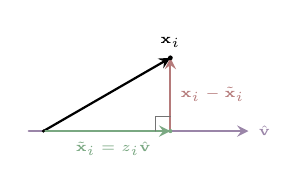
\begin{tikzpicture}[scale=0.62, line cap=round, >=stealth]
        \draw[softPurple, thick, ->] (-0.3,0) -- (4.2,0) node[right, font=\tiny] {$\hat{\mathbf{v}}$};
        \coordinate (O) at (0,0);
        \coordinate (xi) at (2.6,1.5);
        \coordinate (px) at (2.6,0);
        \draw[black, thick, ->] (O) -- (xi) node[above, font=\tiny] {$\x_i$};
        \draw[softGreen, thick, ->] (O) -- (px) node[below, font=\tiny, pos=0.55] {$\tilde{\x}_i = z_i\hat{\mathbf{v}}$};
        \draw[softRed, thick, ->] (px) -- (xi) node[right, font=\tiny, midway] {$\x_i-\tilde{\x}_i$};
        \draw[black!55, line width=0.3pt] (2.3,0) -- (2.3,0.3) -- (2.6,0.3);
        \fill (xi) circle (1.4pt);
        \fill[softGreen] (px) circle (1.2pt);
        \fill (O) circle (1.0pt);
    \end{tikzpicture}
    \end{center}
\end{tcolorbox}

% AUTOENCODERS
\begin{tcolorbox}[formulabox=Autoencoders, colframe=softRed]
    \textbf{AE determinístico}: $\z=f_\phi(\x)$, $\hat{\x}=g_\theta(\z)$, $L\ll D$\\
    $\Loss_\text{AE} = \tfrac{1}{N}\sum_n\|\x_n - g_\theta(f_\phi(\x_n))\|^2$\\
    \textbf{AE lineal} $\equiv$ PCA (mismo subespacio); con no-linealidades $\to$ reducción no-lineal.\\[2pt]
    \vspace{-2mm}
    \tcbline
    \vspace{-2mm}
    \textbf{VAE}: prior $p(\z)=\mathcal{N}(\mathbf{0},\mathbf{I})$\\
    Encoder: $q_\phi(\z|\x)=\mathcal{N}(\z|\muu_\phi(\x),\text{diag}(\boldsymbol{\sigma}^2_\phi(\x)))$\\
    Decoder: $p_\theta(\x |\z)=\mathcal{N}(\x |f_d(\z;\theta), \sigma^2\mathbf{I})$\\[2pt]
    \textbf{ELBO} (a maximizar):\\
    $\Loss_\text{VAE} = \mathbb{E}_{q_\phi}[\ln p_\theta(\x|\z)] - \text{KL}(q_\phi(\z|\x)\|p(\z))$\\
    \textbf{KL gaussiano}:\\
    $\text{KL}(\mathcal{N}(\muu,\text{diag}(\boldsymbol{\sigma}^2))\|\mathcal{N}(\mathbf{0},\mathbf{I}))$\\
    $= \tfrac{1}{2}\sum_j(\mu_j^2+\sigma_j^2-\ln\sigma_j^2-1)$\\[2pt]
    \textbf{Reparam.}: $\z=\muu_\phi(\x)+\boldsymbol{\sigma}_\phi(\x)\odot\boldsymbol{\varepsilon}$, $\boldsymbol{\varepsilon}\sim\mathcal{N}(\mathbf{0},\mathbf{I})$\\
    \textbf{Forward}: $\x\to f_e\to \underset{\Loss_{KL}}{(\muu,\boldsymbol{\sigma}})\to\z\to f_d \to \underset{\Loss_\text{rec}}{\hat{\x}}$\\
    \textbf{Backward}: $\overset{\Loss_\text{rec}}{\nabla_\theta f_d} \to \overset{\Loss_{KL}}{\nabla(\muu,\boldsymbol{\sigma})}\to \nabla_\phi f_e \to \nabla \Loss$\\
    $\nabla \Loss \begin{cases}\nabla_\theta\Loss=\nabla_\theta\Loss_\text{rec} \\ \nabla_\phi\Loss=\nabla_\phi\Loss_\text{rec}+\nabla_\phi\Loss_\text{KL}\end{cases}$
\end{tcolorbox}

% INFORMATION THEORY
\begin{tcolorbox}[formulabox=Information Theory, colframe=softTeal]
    \textbf{Entropía}: $\mathbb{H}(p) = -\sum_i p_i\log p_i \geq 0$\\
    \textbf{KL divergence} (no simétrica, $\geq 0$):\\
    $D_\mathbb{KL}(q\|p) = \sum_i q_i\ln\tfrac{q_i}{p_i} = \mathbb{E}_q\!\left[\ln\tfrac{q}{p}\right]$\\
    $D_\mathbb{KL}(q\|p)=0 \Leftrightarrow q=p$;\quad $D_\mathbb{KL}(q\|p)\neq D_\mathbb{KL}(p\|q)$\\[2pt]
    \textbf{KL gaussianas} ($p=\mathcal{N}(\muu_1,\Sig_1)$, $q=\mathcal{N}(\muu_0,\Sig_0)$):\\
    $D_\mathbb{KL}(q\|p)=\tfrac{1}{2}\!\big[\ln\tfrac{|\Sig_1|}{|\Sig_0|}+\text{tr}(\Sig_1^{-1}\Sig_0)$ \\ 
    $\phantom{D_\mathbb{KL}(q\|p)=}+(\muu_1{-}\muu_0)^\top\Sig_1^{-1}(\muu_1{-}\muu_0)-D\big]$\\
    Caso $p=\mathcal{N}(\mathbf{0},\mathbf{I})$: $D_\mathbb{KL}=\tfrac{1}{2}\sum_j(\mu_j^2+\sigma_j^2-\ln\sigma_j^2-1)$\\[2pt]
\end{tcolorbox}

% CLUSTERING METRICS
\begin{tcolorbox}[formulabox=Métricas de Clustering, colframe=softGreen]
    $\underset{\text{within}}{\text{WCSS}} = \sum_k\sum_{n:r_{nk}=1}\|\x_n-\muu_k\|^2$ ($\downarrow$ mejor)\\
    $\underset{\text{between}}{\text{BCSS}} = \sum_k N_k\|\muu_k-\bar{\x}\|^2$ ($\uparrow$ mejor)\\[2pt]
    \textbf{Silhouette} $s(n)\in[-1,1]$: $a(n)$ = dist.\ intra, $b(n)$ = dist.\ al vecino más cercano\\
    $s(n)=\tfrac{b(n)-a(n)}{\max(a(n),b(n))}$;\quad $\bar{s}=\tfrac{1}{N}\sum_n s(n)$\\[2pt]
    \textbf{Davies-Bouldin}: $\text{DB}=\tfrac{1}{K}\sum_k\max_{k'\neq k}\tfrac{s_k+s_{k'}}{d(\muu_k,\muu_{k'})}$\\
    \textbf{Elbow}: graficar WCSS vs.\ $K$; codo $= K$ óptimo.\\
    \textbf{BIC}: $-2\ln\hat{p}(\X) + d_K\ln N$; $\downarrow$ mejor; selecciona $K$.
    \textbf{Mutual. Info} (con labels):\\
    $I(S_k;Y)=\sum_i\sum_j p_{C_iY}(i,j)\log\dfrac{p_{C_iY}(i,j)}{p_{C_i}(i)\,p_Y(j)}$\\
    $p_{C_iY}(i,j)=\tfrac{|c_i\cap y_j|}{N}$;\quad $I(X;Y)=0\Leftrightarrow X\perp Y$\\
    $I(X;Y)=\mathbb{H}(X)-\mathbb{H}(X|Y)=\mathbb{H}(Y)-\mathbb{H}(Y|X)$\\[2pt]
    \textbf{NMI} (Normalized Mutual Information):\\
    $\text{NMI}(S_k,Y)=\dfrac{2\,I(S_k;Y)}{\mathbb{H}(S_k)+\mathbb{H}(Y)}\in[0,1]$\quad($\uparrow$ mejor)
\end{tcolorbox}

% DEMO 2
\begin{tcolorbox}[formulabox={Demo: PCA invariante roto-traslaciones}, colframe=softBrown]
    $\x_i'= R\x_i + \bias$\\
    \textbf{Traslación}: $\x_i'=\x + \bias \implies \muu' = \muu + \bias$.\\
    $\tilde{\x}=\x'_i - \muu'  = \x_i + \bias - (\muu+ \bias) = \x_i - \muu$.\\
    \textbf{Rotación}: $\tilde{\x}_i' = \mathbf{R}\tilde{\x}_i$, $\mathbf{R}$ de rotación ($\perp$, $\det = 1$). \\
    $\hat{\Sig}' = \mathbf{R}\tilde{\X}\tilde{\X}^\top\mathbf{R}^\top = \mathbf{R}\hat{\Sig}\mathbf{R}^\top$\\
    Si $\hat{\Sig}\mathbf{u}_l=\lambda_l\mathbf{u}_l$ $\Rightarrow$ $\hat{\Sig}'(\mathbf{R}\mathbf{u}_l)=\lambda_l(\mathbf{R}\mathbf{u}_l)$\\
    Coords reducidas: $z_l' = (\mathbf{R}\mathbf{u}_l)^\top(\mathbf{R}\tilde{\x}_i) = \mathbf{u}_l^\top\mathbf{R}^\top\mathbf{R}\tilde{\x}_i = z_l$.
\end{tcolorbox}
 
% DEMO 4
\begin{tcolorbox}[formulabox={Demo: PCA: $\max \mathbb{V}[\z] \equiv \min \tfrac{1}{N}\|\x-\tilde{\x}\|^2$}, colframe=softBrown]
    $\bar{\z} = \tfrac{1}{N}\sum z_i = \bar{\x}^T \hat{v}=0 \implies \mathbb{V}[\z]=\tfrac{1}{N}\sum z_i^2$
    \begin{align*}
        \min_{\hat{v}} \tfrac{1}{N}\sum\|x_i-z_i\hat{v}\|^2 &\equiv \max_{\hat{v}} \tfrac{1}{N}\sum z_i^2 \\
        \min_{\hat{v}} \tfrac{1}{N}\sum \|x_i\|^2- z_i^2 &\equiv \max_{\hat{v}} \tfrac{1}{N}\sum z_i^2 \\
        \min_{\hat{v}} -\tfrac{1}{N}\sum z_i^2 &\equiv \max_{\hat{v}} \tfrac{1}{N}\sum z_i^2
    \end{align*}
\end{tcolorbox}

\end{minipage}
\hfill
%%%%%%%%%%%%%%%%%%%%%%%%%%%%%%%%%%%%%%% COL 3 %%%%%%%%%%%%%%%%%%%%%%%%%%%%%%%%%%%%%%%
\begin{minipage}[t]{0.3299\textwidth}
\vspace{0pt}

% DBSCAN
\begin{tcolorbox}[formulabox=Clustering+, colframe=softRed]
    \textbf{HAC} (Hierarchical Agglomerative):\\
    Bottom-up: empieza con $N$ clusters, fusiona iterativamente los más cercanos $\to$ dendrograma. No requiere $K$ a priori.\\
    \textit{Linkage}: single ($\min$ dist), complete ($\max$ dist), average, Ward ($\min\Delta$WCSS).\\[2pt]
    \textbf{DBSCAN}: params $\varepsilon$, MinPts.\\
    \textit{Core}: $|\mathcal{N}_\varepsilon(\x)|\geq\text{MinPts}$;\; \textit{Border}: vecino de core; \textit{Noise}: resto.\\
    Clusters = componentes conexas de cores + borders.
    \begin{algorithmic}[0]
        \For{$\x_n$ no visitado}
            \If{$|\mathcal{N}_\varepsilon(\x_n)|\geq\text{MinPts}$} nuevo cluster; expandir($\x_n$)
            \Else\ noise \EndIf
        \EndFor
    \end{algorithmic}
    No requiere $K$; detecta formas arbitrarias; sensible a $\varepsilon$.\\[2pt]
    \textbf{Spectral Clustering}:\\
    Grafo de similitud $\mathbf{W}$; Laplaciano $\mathbf{L}=\mathbf{D}-\mathbf{W}$.\\
    Usar los $K$ autovectores de menor $\lambda$ de $\mathbf{L}$ como features; aplicar K-Means. Detecta clusters no convexos.\\[2pt]
    \textbf{Mixture of Bernoullis} ($\x\in\{0,1\}^D$):\\
    $p(\x|\w)=\sum_k\pi_k\prod_d\mu_{kd}^{x_d}(1{-}\mu_{kd})^{1-x_d}$\\
    EM igual que GMM; M-step: $\hat{\mu}_{kd}=\tfrac{\sum_n r_{nk}x_{nd}}{N_k}$
\end{tcolorbox}

% LINALG
\begin{tcolorbox}[formulabox=Álgebra Lineal, colframe=softOrange]
    \textbf{Traza y ciclo}: $\text{tr}(\mathbf{ABC})=\text{tr}(\mathbf{CAB})=\text{tr}(\mathbf{BCA})$\\
    $\x^\top\mathbf{A}\x = \text{tr}(\mathbf{A}\x\x^\top)$ \quad (escalar $\to$ traza)\\[2pt]
    \textbf{Gradientes matriciales clave}:\\
    $\nabla_\mathbf{A}\text{tr}(\mathbf{A}\mathbf{B}) = \mathbf{B}^\top$\\
    $\nabla_\mathbf{A}\ln|\mathbf{A}| = \mathbf{A}^{-\top}$ (i.e.\ $\Sig^{-1}$ si $\Sig$ SDP)\\
    $\nabla_\mathbf{A}(\x^\top\mathbf{A}^{-1}\x) = -\mathbf{A}^{-\top}\x\x^\top\mathbf{A}^{-\top}$\\[2pt]
    \textbf{Identidades para $\Sig$} (sugeridas en ej.\ 20):\\
    Si $\Lambda=\Sig^{-1}$: $\nabla_\Lambda\ln|\Lambda|=\Lambda^{-\top}=\Sig^\top$\\
    $\nabla_\Lambda\text{tr}(\Lambda\mathbf{S}) = \mathbf{S}^\top$\\[2pt]
    \textbf{Proyección ortogonal}: $\mathbf{P}=\hat{\mathbf{v}}\hat{\mathbf{v}}^\top$ (rango 1, idempotente)\\
    $\|\x - \mathbf{P}\x\|^2 = \|\x\|^2 - (\x^\top\hat{\mathbf{v}})^2$\\[2pt]
    \textbf{Matriz ortogonal} $\mathbf{R}$: $\mathbf{R}^\top\mathbf{R}=\mathbf{I}$, $|\det\mathbf{R}|=1$\\
    $\|\mathbf{R}\x\|^2 = \x^\top\mathbf{R}^\top\mathbf{R}\x = \|\x\|^2$ (isometría)\\[2pt]
    \textbf{Autovalores y traza/det}:\\
    $\text{tr}(\mathbf{A})=\sum_i\lambda_i$;\quad $|\mathbf{A}|=\prod_i\lambda_i$\\
    $\text{tr}(\mathbf{AB})=\text{tr}(\mathbf{BA})$ incluso si $\mathbf{A},\mathbf{B}$ no cuadradas\\[2pt]
    \textbf{Restricción con Lagrange}: \\
    $\max_{\hat{\mathbf{v}}}\hat{\mathbf{v}}^\top\hat{\Sig}\hat{\mathbf{v}}$ s.t.\ $\|\hat{\mathbf{v}}\|=1$\\
    $\Rightarrow \mathcal{L} = \hat{\mathbf{v}}^\top\hat{\Sig}\hat{\mathbf{v}} - \lambda(\hat{\mathbf{v}}^\top\hat{\mathbf{v}}-1)$\\
    $\Rightarrow \hat{\Sig}\hat{\mathbf{v}}=\lambda\hat{\mathbf{v}}$ (autoproblema)\\
    $\Rightarrow$ máx.\ varianza $= \lambda_1$ con $\hat{\mathbf{v}}=\mathbf{u}_1$\\
    \textbf{Gaussiana multivariada} $\mathcal{N}(\x|\muu,\Sig)$:\\
    $\dfrac{1}{(2\pi)^{D/2}|\Sig|^{1/2}}\exp\!\left(-\tfrac{1}{2}(\x{-}\muu)^\top\Sig^{-1}(\x{-}\muu)\right)$\\
\end{tcolorbox}

% DEMO 6
\begin{tcolorbox}[formulabox={Demo: EM-GMM - $Q$ y concavidad}, colframe=softBrown]
    \textbf{E-step} — $\mathcal{Q}(\w,\w^\text{old})$:\\
    $p(\X,\mathbf{Z}|\w)=\prod_n\prod_k[\pi_k\mathcal{N}(\x_n|\muu_k,\Sig_k)]^{z_{nk}}$\\
    $\ln p(\X,\mathbf{Z}|\w)=\sum_n\sum_k z_{nk}[\ln\pi_k+\ln\mathcal{N}(\x_n|\muu_k,\Sig_k)]$\\
    $\mathcal{Q}=\sum_n\sum_k r_{nk}[\ln\pi_k - \tfrac{1}{2}\ln|\Sig_k| - \tfrac{1}{2}(\x_n{-}\muu_k)^\top\Sig_k^{-1}(\x_n{-}\muu_k)]$\\[2pt]
    \textbf{M-step} para $\muu_k$: $\nabla_{\muu_k}\mathcal{Q}=0$\\
    $\sum_n r_{nk}\Sig_k^{-1}(\x_n{-}\muu_k)=0 \Rightarrow \hat{\muu}_k = \tfrac{\sum_n r_{nk}\x_n}{N_k}$\\[2pt]
    \textbf{M-step} para $\Sig_k$: $\nabla_{\Lambda_k}\mathcal{Q}=0$ con $\Lambda_k=\Sig_k^{-1}$:\\
    $\tfrac{N_k}{2}\Sig_k - \tfrac{1}{2}\sum_n r_{nk}(\x_n{-}\hat{\muu}_k)(\x_n{-}\hat{\muu}_k)^\top=0$\\
    $\Rightarrow \hat{\Sig}_k = \tfrac{1}{N_k}\sum_n r_{nk}(\x_n{-}\hat{\muu}_k)(\x_n{-}\hat{\muu}_k)^\top$\\[2pt]
    \textbf{M-step} para $\pi_k$ (Lagrange $\sum\pi_k=1$):\\
    $\nabla_{\pi_k}[\mathcal{Q}+\nu(\sum\pi_k-1)]=0 \Rightarrow \hat{\pi}_k=\tfrac{N_k}{N}$\\[2pt]
    \textbf{Concavidad de $\mathcal{Q}$}: es una suma de $\ln\mathcal{N}$ ponderados; $\ln\mathcal{N}$ es cóncavo en $(\muu_k,\Sig_k)$ $\Rightarrow$ $\mathcal{Q}$ cóncava $\Rightarrow$ M-step es único. $\square$
\end{tcolorbox}

% DEMO 1
\begin{tcolorbox}[formulabox={Demo: PCA minimiza error de recon.}, colframe=softBrown]
    Datos centrados ($\hat{\muu}=0$). $\tilde{x}_i = z_i\hat{\mathbf{v}}$, $z_i = \x_i^\top\hat{\mathbf{v}}$.\\
    $\text{MSE} = \tfrac{1}{N}\sum_i\|\x_i - z_i\hat{\mathbf{v}}\|^2$\\
    $= \tfrac{1}{N}\sum_i\|\x_i\|^2 - \tfrac{1}{N}\sum_i(\x_i^\top\hat{\mathbf{v}})^2$\\
    $= \text{const} - \hat{\mathbf{v}}^\top\!\left(\tfrac{1}{N}\X^\top\X\right)\!\hat{\mathbf{v}}$\\
    $\Rightarrow$ minimizar MSE $\equiv$ maximizar $\hat{\mathbf{v}}^\top\hat{\Sig}\hat{\mathbf{v}}$.\\
    Con restricción $\|\hat{\mathbf{v}}\|=1$ (Lagrange):\\
    $\hat{\Sig}\hat{\mathbf{v}}=\lambda\hat{\mathbf{v}}$; la varianza $=\lambda$.\\
    $\Rightarrow \hat{\mathbf{v}}^*=\mathbf{u}_1$ (autovector de $\lambda_{\max}$).
\end{tcolorbox}

% DEMO 5
\begin{tcolorbox}[formulabox={Demo: GMM: +K $\implies$ log-lik no decrece}, colframe=softBrown]
    Sea $\w_K^*$ óptimo para $K$ clusters. Construir modelo con $K{+}1$ clusters tomando $\w_{K+1}$ con $\pi_{K+1}=0$.\\
    $\Rightarrow p_{K+1}(\X|\w_{K+1}) = p_K(\X|\w_K^*)$\\
    $\Rightarrow \ln p(\X|\w_{K+1}^*) \geq \ln p(\X|\w_{K+1}) = \ln p(\X|\w_K^*)$
\end{tcolorbox}

\end{minipage}

\end{document}